%!TEX root = ../thesis.tex
\section{Client: Entwurf und Implementierung}

{\draft Hier etwas über komponentenbasierten Ansatz für Design \& Programmierung}

\subsection{Grunlagen zum Entwurf des User Interfaces}

Das User Interface der Webanwendung besteht aus verschiedenen \emph{Screens}. Ein Screen lässt sich umgangssprachlich als ``Unterseite'' beschreiben. Für den Nutzer sind vor allem drei Screens wichtig:

\begin{itemize}
  \item Chronologische Auflistung aller Builds (Historie)
  \item Übersicht des letzten Builds je Pipeline (neueste Builds)
  \item Einzelansicht eines Build-Prozesses (Detail)
\end{itemize}

Screens mit Formularen wurden außen vor gelassen, beispielsweise zum Erstellen einer Pipeline.

\subsubsection{Content Inventory}

Ein \emph{Content Inventory}\footnote{https://github.com/north/north\#content-inventory} ist eine Auflistung aller verfügbarer Daten. Beim Designprozess hilft es dabei, einen Überblick über alle zu verwendenden Daten zu behalten und Prioritäten herauszuarbeiten.

In Tabelle \ref{tab:content-inventory} ist das Content Inventory auf die wichtigsten anzuzeigenden Komponenten bzw. Entitäten aufgeteilt.

\begin{table}[H]
  \scriptsize
  \begin{tabularx}{\textwidth}{| l | p{3cm} | l | X |}
    \hline
    \textbf{Objekt} & \textbf{Attribut} & \textbf{Typ} & \textbf{Notiz} \\ \hline
    \multirow{2}{*}{Projekt} & Titel & text &  \\ \cline{2-4}
      & Git URL & text & Nicht zwingend anzuzeigen \\ \hline
    \multirow{3}{*}{Pipeline} & Titel & text &  \\ \cline{2-4}
      & Bezeichner & text & Für Zuordnung in .warp.yml \\ \cline{2-4}
      & Regex-Auslöser & text &   \\ \hline
    \multirow{13}{*}{Build-Prozess} & Titel & text & Titel der Pipeline \\ \cline{2-4}
      & Nummer & integer &  \\ \cline{2-4}
      & Status & enum & queued, init, active, success, failed, stopped \\ \cline{2-4}
      & Startzeit & datetime &  \\ \cline{2-4}
      & Endzeit & datetime & bei aktivem Prozess nicht vorhanden \\ \cline{2-4}
      & Dauer & time & Ergibt sich aus Start- und Endzeit \\ \cline{2-4}
      & Durchschnittliche Dauer & time &  \\ \cline{2-4}
      & Differenz: Dauer und Durchschnittliche Dauer & time &  \\ \cline{2-4}
      & Git Reference & text & Branch oder Tag \\ \cline{2-4}
      & Commit SHA & text &  \\ \cline{2-4}
      & Commit Nachricht & long text & Kann mehrere Zeilen lang sein, sollte gekürzt werden \\ \cline{2-4}
      & User Bild & image & quadratisch \\ \cline{2-4}
      & User Name & text &  \\ \hline
    \multirow{5}{*}{Stage} & Titel & text &  \\ \cline{2-4}
      & Nummer & integer & Fortlaufende Nummerierung der Stages \\ \cline{2-4}
      & Status & enum & queued, init, active, success, failed, stopped \\ \cline{2-4}
      & Startzeit & datetime &  \\ \cline{2-4}
      & Endzeit & datetime & bei aktiver Stage nicht vorhanden \\ \cline{2-4}
      & Dauer & time & Ergibt sich aus Start- und Endzeit \\ \hline
    \multirow{5}{*}{Step} & Titel & text &  \\ \cline{2-4}
      & Befehl & text &  \\ \cline{2-4}
      & Status & enum & queued, init, active, success, failed, stopped \\ \cline{2-4}
      & Startzeit & datetime &  \\ \cline{2-4}
      & Endzeit & datetime & bei aktiver Stage nicht vorhanden \\ \cline{2-4}
      & Dauer & time & Ergibt sich aus Start- und Endzeit \\ \cline{2-4}
      & Ausgabe & long text & kann sehr lang werden \\ \hline
  \end{tabularx}
  \caption{Content Inventory}
  \label{tab:content-inventory}
\end{table}

\subsection{Visualisierung der Build-Historie}
\label{subsec:visualisierung-build-history}

Die Historie ist eine chronologische Auflistung aller Builds des Projekts. Aus ihr wird schnell ersichtlich, wann es zu Fehlern kam und wann diese behoben wurden. Viele Details zum einzelnen Build-Prozess sind daher nicht notwendig.

\begin{figure}[h]
  \caption{Kompakte Build-Prozess Komponenten mit positivem und negativem Status}
  \label{fig:build-process-short}
  \centering
    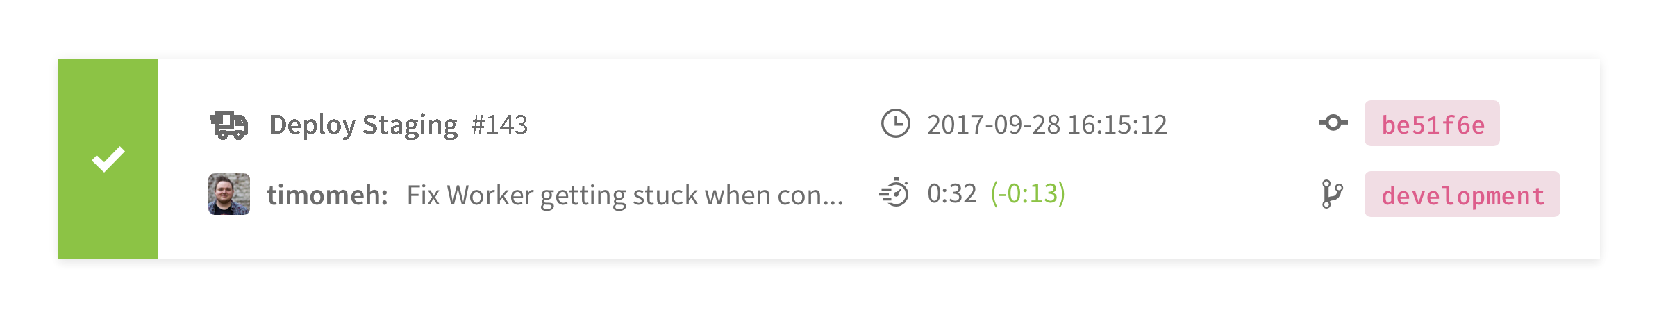
\includegraphics[width=\textwidth]{assets/build-overview-finished}
    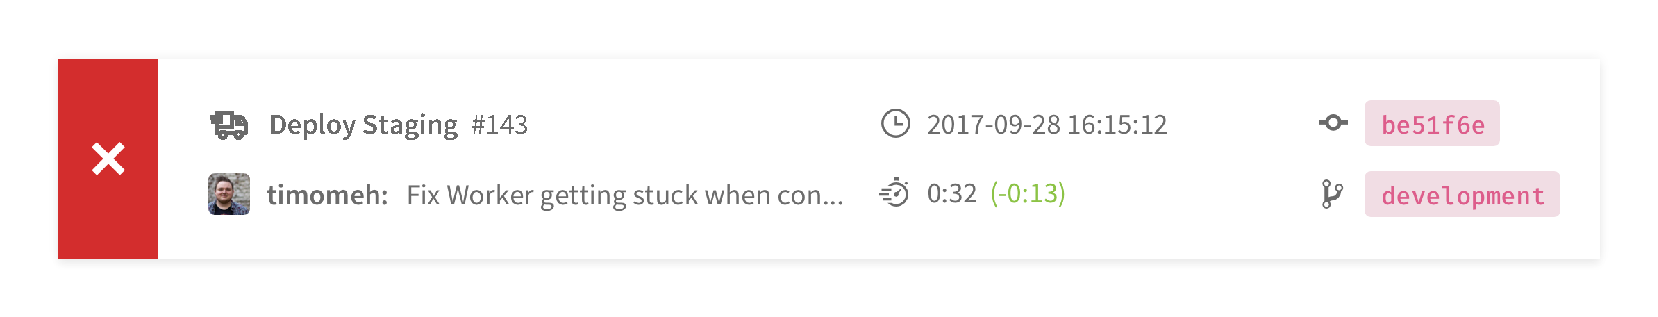
\includegraphics[width=\textwidth]{assets/build-overview-failed}
\end{figure}

Zu den wichtigsten Informationen eines Build-Prozesses gehört sein Status. Daher ist der Status in der Komponente aus Abbildung \ref{fig:build-process-short} gut sichtbar links platziert. Weitere Daten in dieser Komponente wurden auf die wichtigsten Informationen reduziert.

Die Informationen wurden auf feste vertikale Ebenen aufgeteilt. Bei der Auflistung entsteht dadurch ein einheitliches Bild ohne visuelle Störungen.

Die Komponente ist nicht sehr hoch, damit mehr Elemente gleichzeitig im Viewport sichtbar sind (siehe Abbildung \ref{fig:build-history}).

\begin{figure}[H]
  \caption{Chronologische Auflistung der Build-Prozesse}
  \label{fig:build-history}
  \centering
    \includegraphics[width=\textwidth]{assets/build-history}
\end{figure}

\subsection{Visualisierung der neuesten Builds}

Die neuesten Builds ist eine der wichtigsten Informationen. Zu jeder Pipeline wird der aktuellste Build-Prozess angezeigt. Daraus wird direkt ersichtlich, ob es aktuell Probleme gibt. Ebenso kann der Nutzer in dieser Übersicht direkt erkennen, welche Version der Software auf welche Umgebung deployed wurde.

Hierfür wird im Vergleich zur Historie (siehe Abschnitt \ref{subsec:visualisierung-build-history}) eine Komponente mit mehr Informationen benötigt.

\begin{figure}[h]
  \caption{Informationsreiche Build-Prozess Komponenten mit positivem Status}
  \label{fig:build-process-detail}
  \centering
    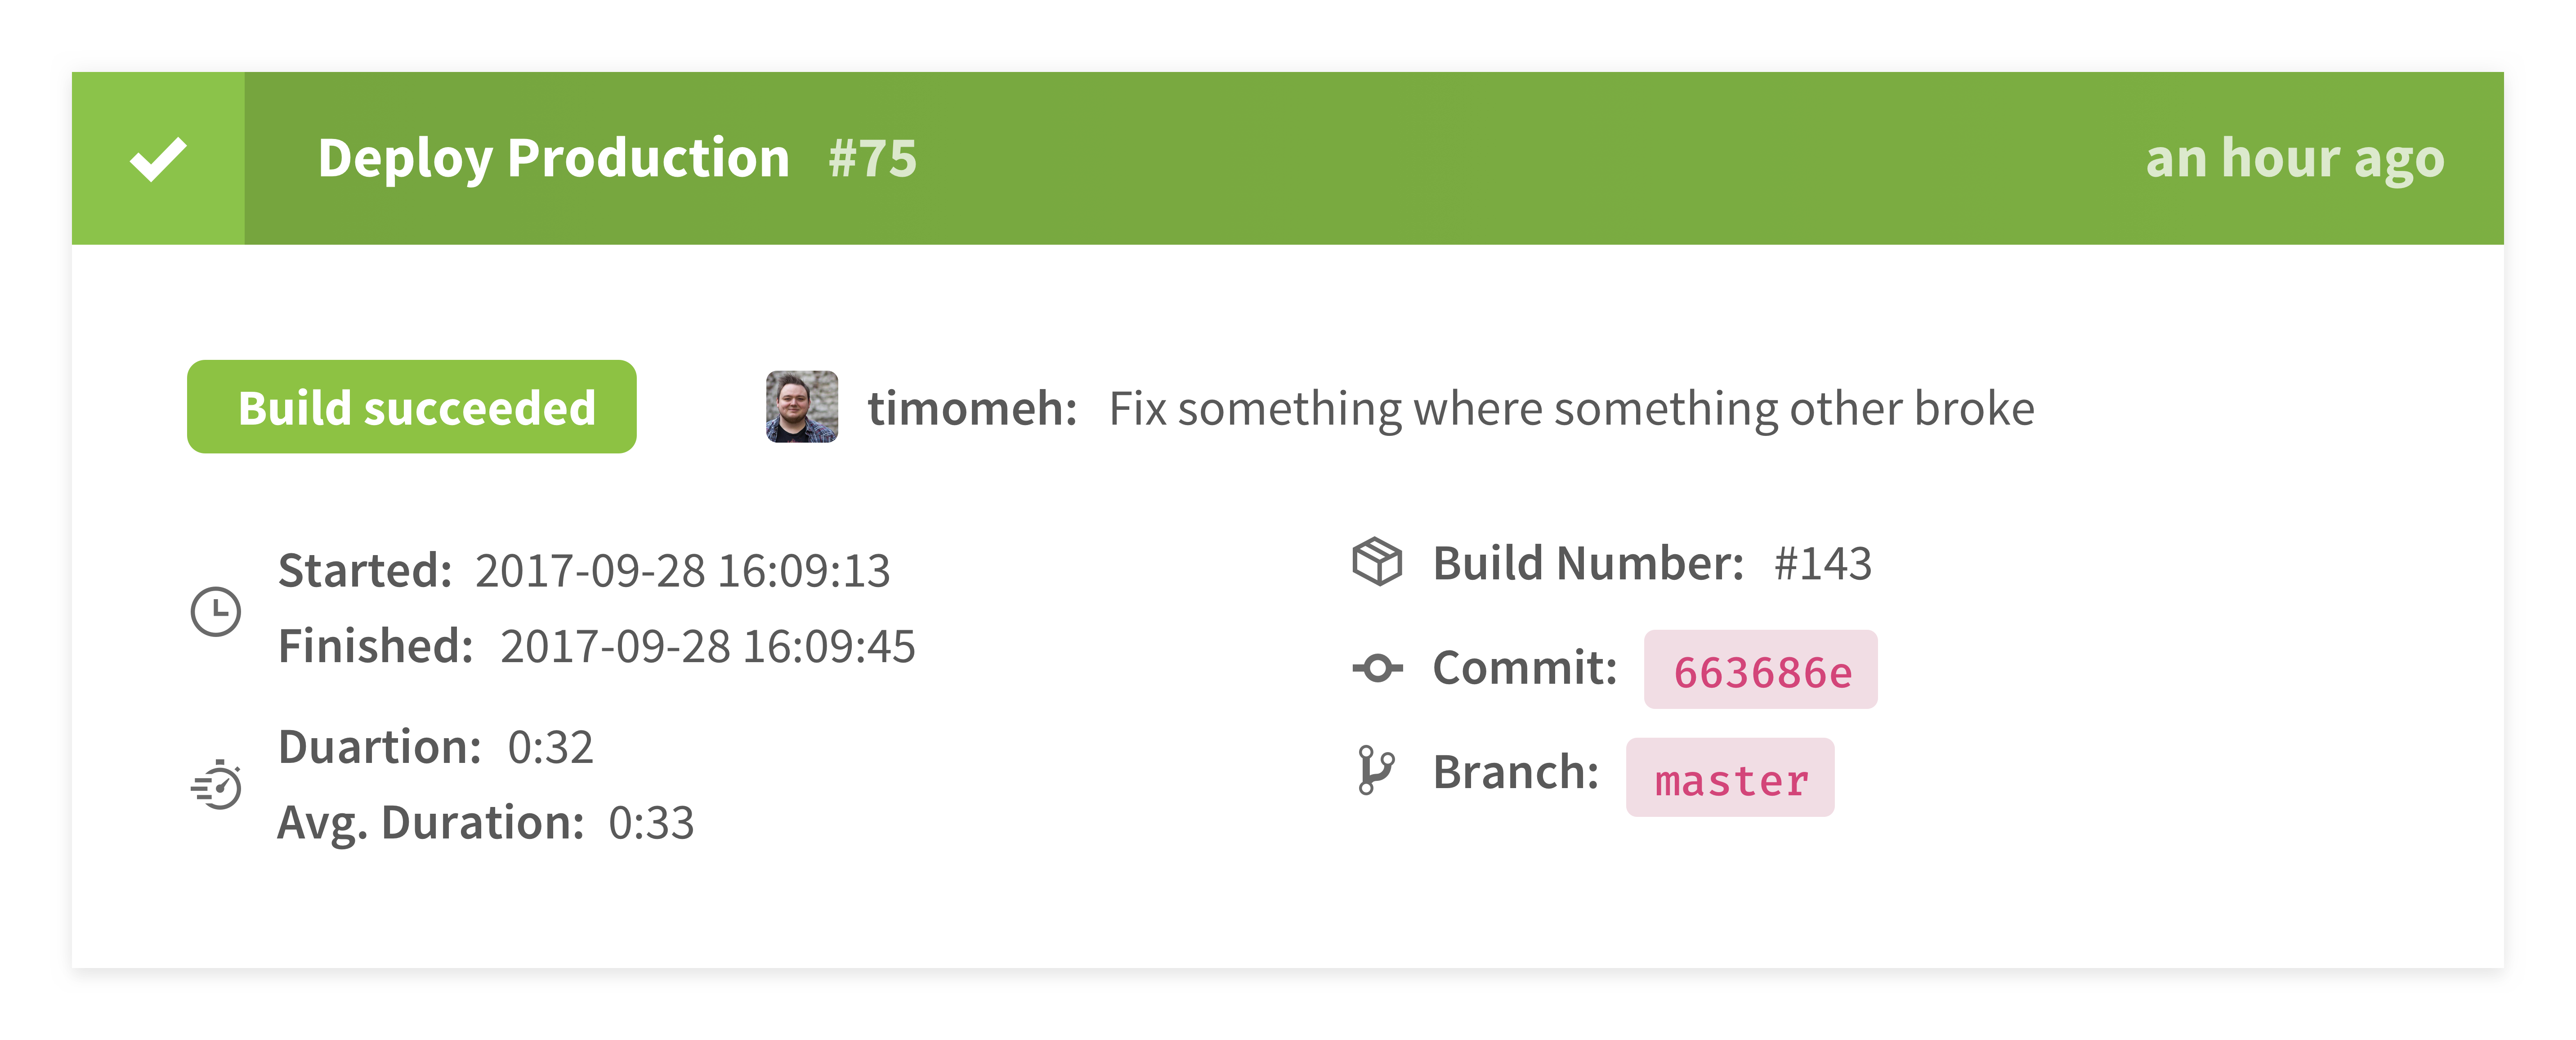
\includegraphics[width=\textwidth]{assets/build-detail-finished}
\end{figure}

Die Komponente in Abbildung \ref{fig:build-process-detail} ist im Vergleich zur kleineren Komponente in Abbildung \ref{fig:build-process-short} anders strukturiert, da der Fokus nicht mehr auf der Auflistung sondern dem einzelnen Build-Prozess liegt. Trotzdem enthält sie visuelle Ähnlichkeiten, damit ein Bezug zwischen beiden Komponenten erkennbar bleibt.

Die Informationen des Build-Prozesses haben neben dem Icon nun auch eine textuelle Bezeichnung, um Verwirrung durch die Masse an Daten zu vermeiden.

Bei einem aktiven Build-Prozess ist an dieser Stelle eine Fortschrittsanzeige sinnvoll. Manche Anwendungen verwenden hierfür einen Ladebalken mit prozentualem Fortschritt. Diese Anzeige ist jedoch irreführend: Nachdem ein Schritt in einem Build-Prozess gestartet wurde, kennt die Anwendung nicht den Fortschritt innerhalb des Schrittes. Sie weiß nur, ob der Befehl gestartet und ob er beendet wurde. Die Anwendung weiß auch nicht, wie lange ein Schritt dauert\footnote{Die Dauer eines Schrittes liese sich schätzen, indem ein Duchschnittswert aus füheren Build-Prozessen errechnet wird.}. Möglicherweise dauert ein bestimmter Schritt um ein vielfaches länger als andere Schritte.

\begin{figure}[h]
  \caption{Informationsreiche Build-Prozess Komponenten mit aktivem Status}
  \label{fig:build-process-detail-active}
  \centering
    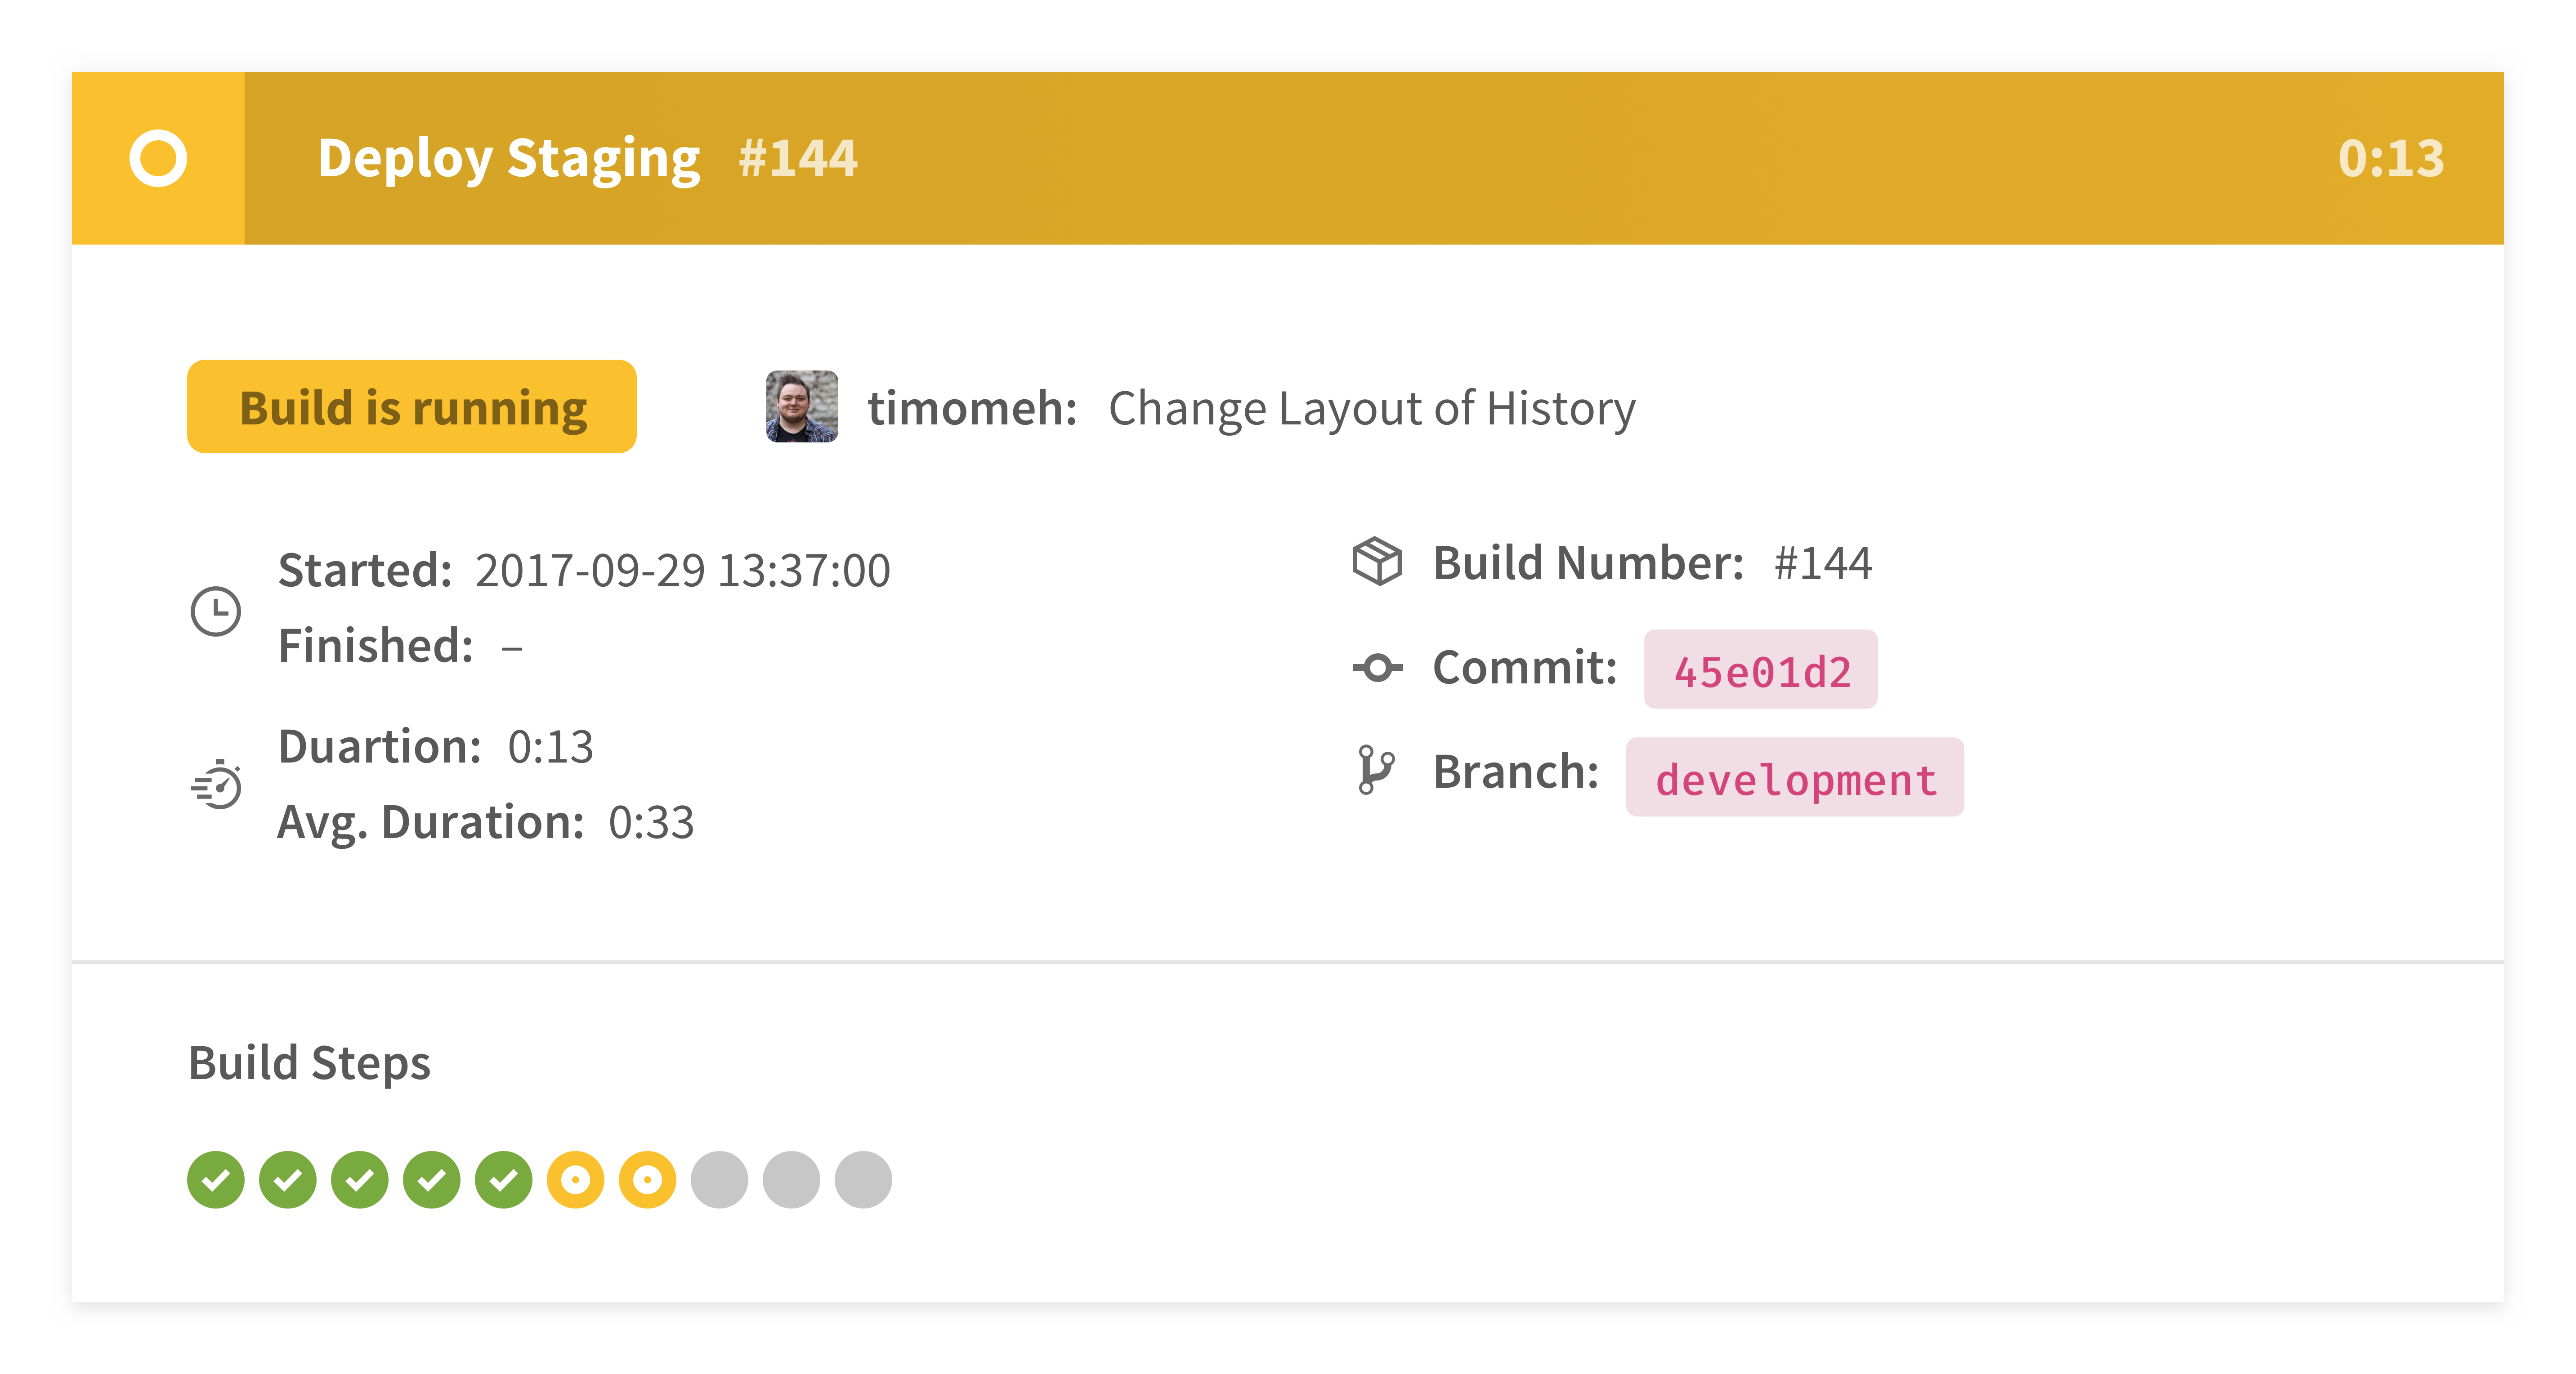
\includegraphics[width=\textwidth]{assets/build-detail-active}
\end{figure}

Daher werden die Schritte auch als solches in vereinfachter Darstellung aufgelistet, wie in Abbildung \ref{fig:build-process-detail-active} zu sehen. Der Nutzer sieht, aus wie vielen Schritten ein Build-Prozess besteht, wie viele davon beendet wurden und wie viele noch ausstehen

Auf dem Screen (siehe Abbildung \ref{fig:latest-builds}) sind diese Komponenten nach Datum absteigend sortiert. Ein größerer Abstand und die deutlich sichtbaren durchgezogenen Farbbalken hilft bei der Trennung der Komponenten voneinander, damit der Fokus auf der einzelne Komponente bleibt.

\begin{figure}[H]
  \caption{Übersicht der neuesten Builds}
  \label{fig:latest-builds}
  \centering
    \includegraphics[width=\textwidth]{assets/latest-builds}
\end{figure}

\subsection{Visualisierung der Pipeline}

Die Visualiserung der gesamten Pipeline (also aller Stages und Abfolge der Schritte des Build-Prozesses) ist für den Nutzer nicht wichtig, wenn ein Build-Prozess erfolgreich war. Erst wenn ein Build-Prozess fehlgeschlagen ist, ist diese Detailansicht zur Fehlererkennung sehr nützlich. In ihr lässt sich erkennen, an welcher Stelle der Build-Prozess fehlgeschlagen ist und was die Ausgabe des fehlgeschlagenen Befehls war.

Die Stärke der Anwendung, dass Schritte beliebig tief in Gruppen verschachtelt werden können, ist gleichzeitig eine Schwäche bei der Visualisierung. Die Pipeline soll übersichtlich und dargestellt werden, was sehr schwierig ist, wenn sich Schritte beliebig aufteilen können und parallele Prozesse entstehen. Zudem soll die Breite des Viewports nicht überschritten werden, wodurch der Nutzer horizontal und vertikal scrollen müsste.

Letztendlich wurde sich für die Visualisierung in Abbildung \ref{fig:pipeline-overview} entschieden, bei der alle Schritte chronologisch untereinander aufgelistet werden, und parallele Prozesse nebeneinander angezeigt werden.

\begin{figure}[h]
  \caption{Einzelansicht des Build-Prozesses}
  \label{fig:pipeline-overview}
  \centering
    \includegraphics[width=\textwidth]{assets/pipeline-overview}
\end{figure}

Um nicht weitere visuelle Elemente einzuführen, wurden Designelemente der Historie (siehe Abschnitt \ref{subsec:visualisierung-build-history}) wiederverwendet.

Ein Nachteil dieser Visualisierung ist, dass bei zu vielen parallelen Prozessen die einzelnen Schritte sehr schmal werden können. Eine Pipeline mit sehr vielen verschachtelten parallelen Prozessen kann allerdings auch ein Anzeichen für einen schlechten Aufbau der Pipeline sein.

\subsection{React und Redux}

\textbf{React} ist eine Bibliothek für JavaScript, mit der sich komponentenbasierte User Interfaces für den Browser programmieren lassen. Wie schon im Praxisprojekt \cite{Maemecke2017} ausgearbeitet, eignet sich React besonders für dynamische Webanwendungen bzw. \acp{SPA} mit komplexen Funktionalitäten.

React wird von Facebook entwickelt und seit 2011 auf facebook.com verwendet. 2013 wurde React als Open-Source-Projekt veröffentlicht. Mittlerweile besitzt React eine sehr große und stetig wachsende Community, und wird auch von vielen Unternehmen und Projekten genutzt. Zu den Bekanntesten zählen u.a. Twitter, Netflix, Paypal, Reddit, Airbnb und viele mehr\footnote{Tatsächlich ist die Verwendung von React aktuell so weit verbreitet, dass eine komplette Auflistung nur der bekanntesten Unternehmen schon den Rahmen sprengen würde.}.

Ein Konzept von React ist der \emph{State}. Im State werden Daten gespeichert, die zur Anzeige des aktuellen Zustands einer Komponente benötigt werden. Jede Komponente kann ihren eigenen State verwalten. Bei großen Anwendungen mit vielen Daten, die in verschiedenen Komponenten benötigt werden, wird die State-Verwaltung in voneinander getrennten Komponenten schnell schwierig. Zur Lösung dieses Problems gibt es die JavaScript-Bibliothek \textbf{Redux}.

Mit Redux lässt sich ein globaler State verwalten, auf den alle Komponenten zugreifen können. Wenn eine Komponente Daten im globalen State modifiziert, werden die Änderungen direkt in allen anderen Komponenten bekannt, die auf diese Daten zugreifen.
